\documentclass{beamer}
\usetheme{Boadilla}

% Override font size limits
\usepackage{anyfontsize}
% Select Computer Concrete as default font
\usepackage{concrete}
% Select Computer Concrete as math font
\usepackage{concmath}
\usepackage[T1]{fontenc}
% Set default font family as serif (sciposter sets sans serif by default)
\renewcommand{\familydefault}{\rmdefault}

\usepackage{xcolor}

\usepackage{amsmath,amssymb}
\newcommand{\earlywarning}{early-warning}
\newcommand{\GW}{{\sc gw}}
\newcommand{\EM}{{\sc em}}
\newcommand{\GRB}{{\sc grb}}
\newcommand{\CBC}{{\sc cbc}}
\newcommand{\LIGO}{{\sc ligo}}
\newcommand{\LCGT}{{\sc lcgt}}
\newcommand{\GEO}{{\sc geo600}}
\newcommand{\ISCO}{{\sc isco}}
\newcommand{\SNR}{{\sc snr}}
\newcommand{\realtime}{real-time}
\newcommand{\Msun}{\ensuremath{M_{\odot}}}
\newcommand{\order}[1]{\ensuremath{\mathcal{O}[#1]}}
\newcommand{\tmpsamps}{\ensuremath{N}}
\newcommand{\numtmps}{\ensuremath{M}}
\newcommand{\numslices}{\ensuremath{S}}
% macros for number of svd basis functions
\newcommand{\SVD}{{\sc svd}}
\newcommand{\svdtmps}[1]{\ensuremath{L^#1}}
\newcommand{\numsvdtmps}{\svdtmps{s}}
% macros for sample points in slices
\newcommand{\slicesamps}[1]{\ensuremath{N^#1}}
\newcommand{\slicessamps}{\slicesamps{s}}
\newcommand{\fftblock}{\ensuremath{D}}
\newcommand{\resampsamps}{\ensuremath{N^\shortdownarrow,\, N^\shortuparrow}}
\newcommand{\fir}{{\sc fir}}
\newcommand{\fft}{{\sc fft}}
\newcommand{\fmax}{\ensuremath{f^0}}
\newcommand{\flops}{flop/s}
\newcommand{\gstlal}{{\tt gstlal}}
\newcommand{\gstreamer}{{\tt GStreamer}}
\newcommand{\numcpus}{{600}}
\newcommand{\lloid}{{\sc lloid}}
\newcommand{\TD}{{\sc td}}
\newcommand{\FD}{{\sc fd}}

% Macros for collapsing sizes of things
% From TUGboat, Volume 22 (2001), No. 4
% http://www.tug.org/TUGboat/tb22-4/tb72perlS.pdf
\def\clap#1{\hbox to 0pt{\hss#1\hss}}
\def\mathllap{\mathpalette\mathllapinternal}
\def\mathrlap{\mathpalette\mathrlapinternal}
\def\mathclap{\mathpalette\mathclapinternal}
\def\mathllapinternal#1#2{\llap{$\mathsurround=0pt#1{#2}$}} 
\def\mathrlapinternal#1#2{\rlap{$\mathsurround=0pt#1{#2}$}} 
\def\mathclapinternal#1#2{\clap{$\mathsurround=0pt#1{#2}$}}

% Colors for signal flow diagram and equation
\def\diagramcolorfir{red}
\def\diagramcolorreconstruct{blue}
\def\diagramcoloraccum{red!50!yellow}

\title[LIGO-Gxxxxxxx-vx]{Toward early-warning detection \\ of compact binary coalescence}
%\subtitle[?]{?}
\institute[LIGO Caltech]{LIGO Laboratory, California Institute of Technology}
\author[L Singer]{\footnotesize{
	Kipp Cannon,
	Romain Cariou,
	Adrian Chapman,
	Mireia Crispin-Ortuzar,
	Nickolas Fotopoulos,
	Melissa Frei,
	Chad Hanna,
	Erin Kara,
	Drew Keppel,
	Laura Liao,
	Stephen Privitera,
	Antony Searle,
	Leo Singer, and
	Alan Weinstein} \\~\\ Presentation by Leo Singer}
\date{August 2, 2011}

\begin{document}


\frame{\titlepage}


\begin{frame}
\frametitle{Introduction}
\end{frame}


\section[Outline]{}
\frame{\tableofcontents}


\section[Motivation]{}


\begin{frame}
\frametitle{Motivation}
\end{frame}


\section[Prospects for early-warning detection]{}


\begin{frame}
	\frametitle{Detectability before merger}
	\begin{columns}
		\begin{column}{0.7\textwidth}
			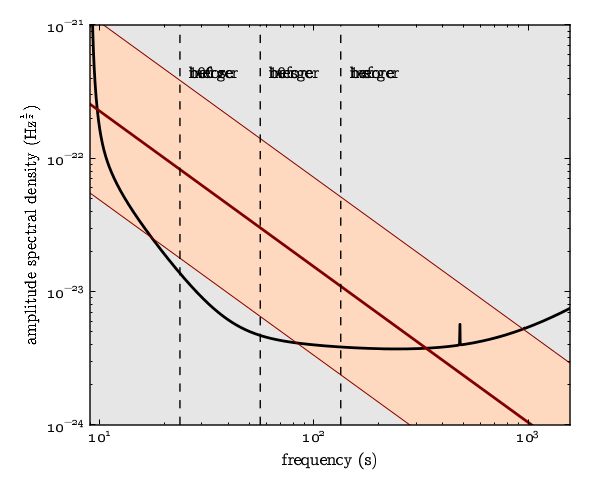
\includegraphics[width=\textwidth]{figures/snr_psd}
		\end{column}
		\begin{column}{0.3\textwidth}
			In advanced \textsc{ligo}, inspiral signals are in principal detectable {\color{ink3}tens or hundreds of seconds} before the \textsc{gw} from the merger have reached the earth.
		\end{column}
	\end{columns}
\end{frame}

\begin{frame}
	\frametitle{Prospects for early-warning detection}
	\begin{center}
		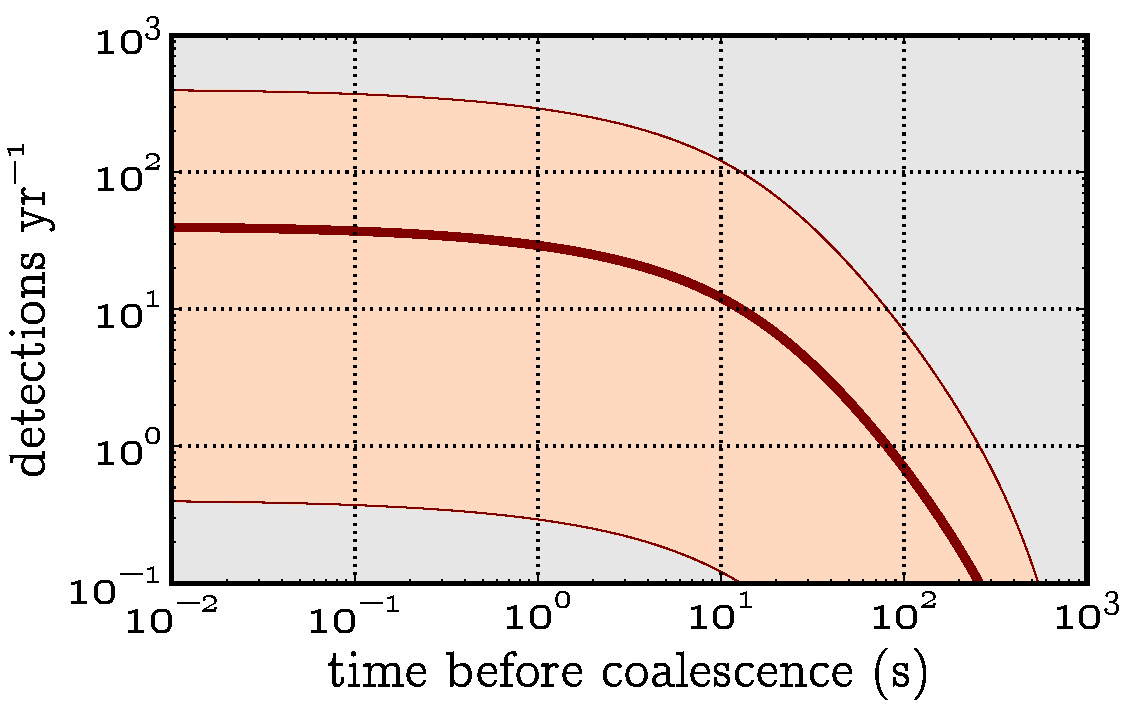
\includegraphics[width=0.7\textwidth]{figures/snr_in_time}
	\end{center}

	Although rates are highly uncertain due to our small sample of confirmed binary neutron stars, of a predicted 40 detections~yr$^{-1}$,
	\begin{itemize}
		\item 10~yr$^{-1}$ will be detectable 10~s before merger, and
		\item 1~yr$^{-1}$ will be detectable 1~s before merger.
	\end{itemize}
\end{frame}

\begin{frame}
	\frametitle{Sky localization accuracy}
	Sky localization accuracy improves rapidly as the signal progresses toward merger.  Although a near real-time \textsc{gw} search pipeline might make it possible to point telescopes minutes after merger, one might hope to image counterparts to a few exceptional events before merger.

	\begin{center}
		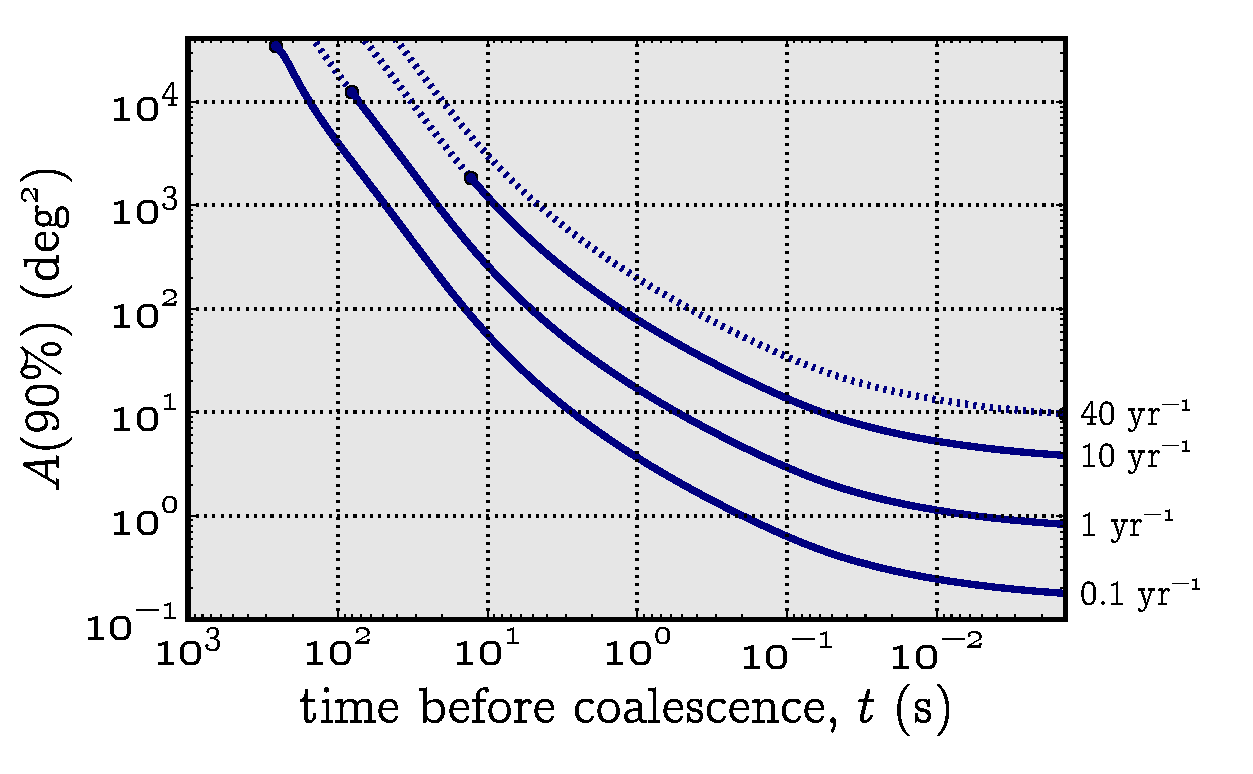
\includegraphics[width=0.75\textwidth]{figures/loc_in_time}
	\end{center}
\end{frame}

\section[Method]{}

\begin{frame}
	\frametitle{Conventional inspiral searches: matched filter banks}
	General relativity predicts the \textsc{gw} signal due to the inspiral of a system with known intrinsic source parameters (mass, eccentricity, spin).
	\\~\\

	\begin{columns}
		\begin{column}{0.5\textwidth}
			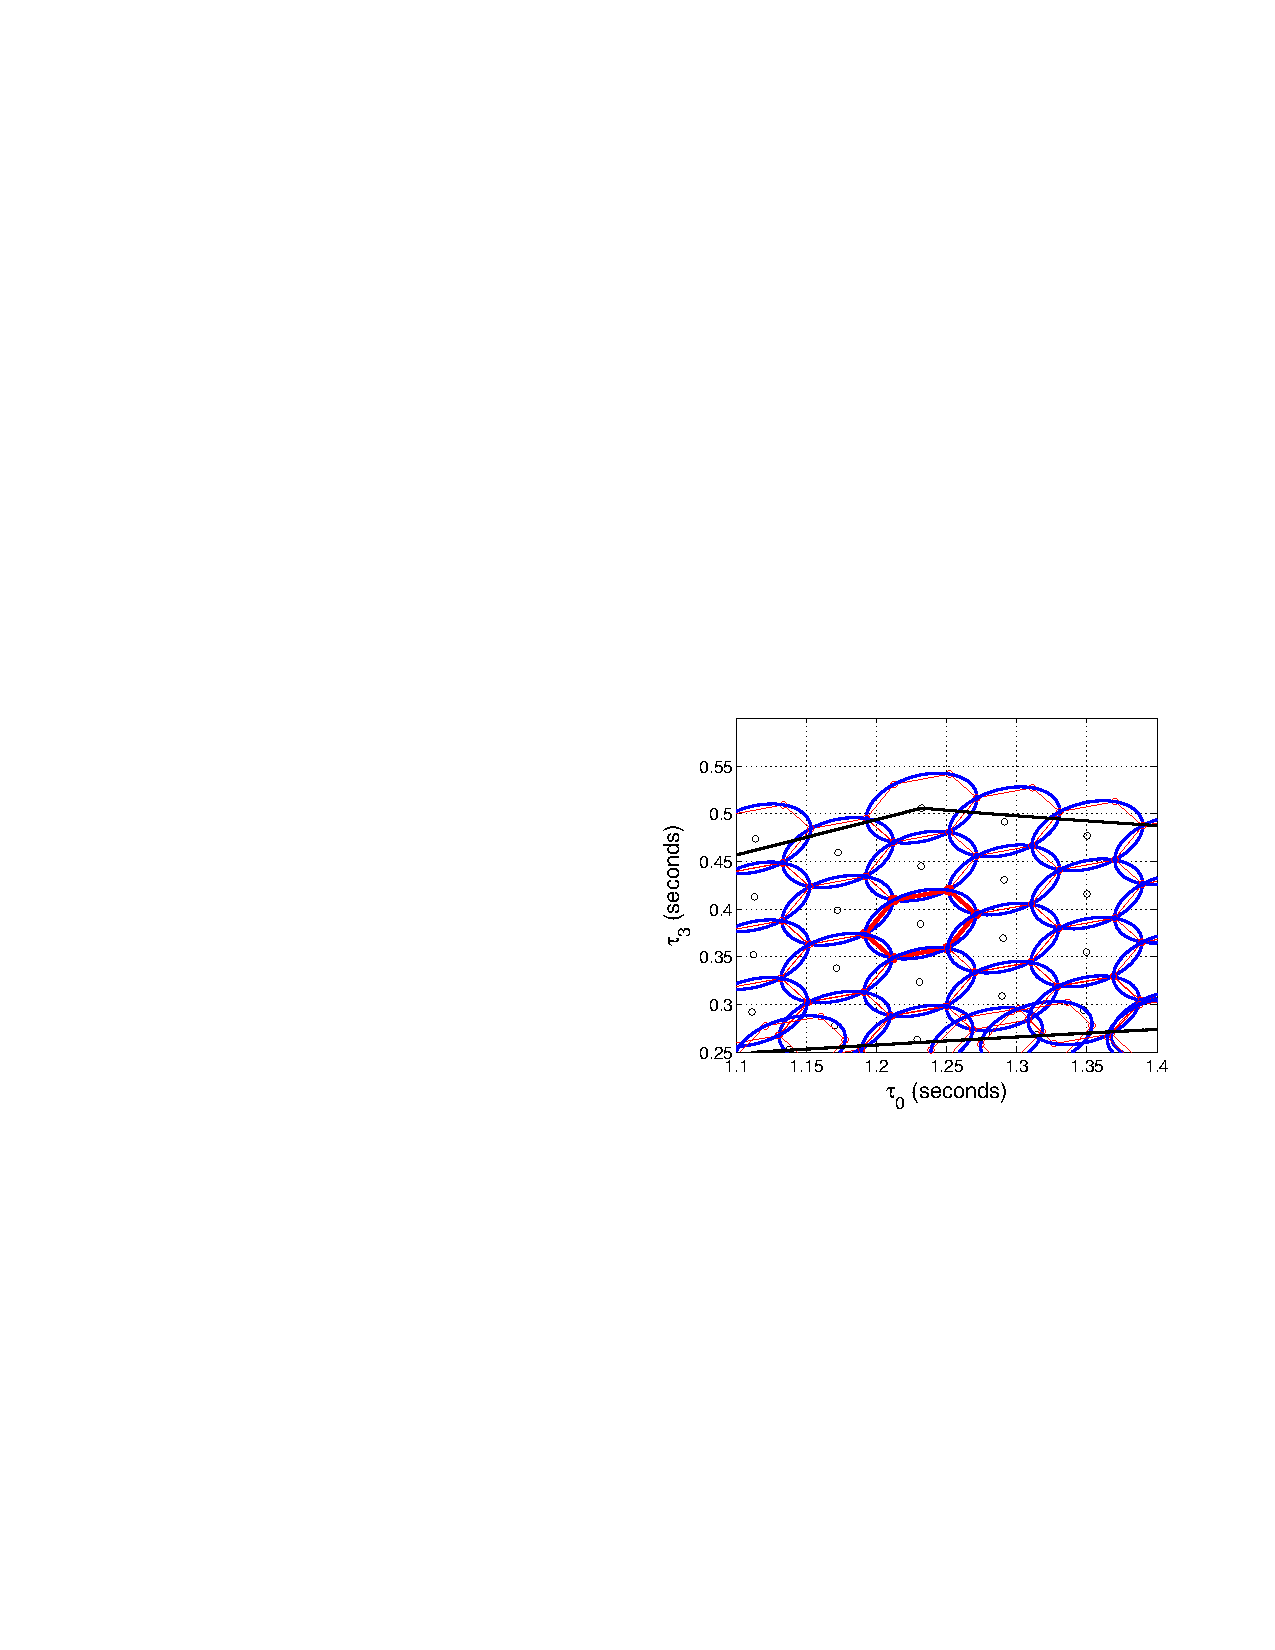
\includegraphics[width=\textwidth]{figures/hexgrid}
		\end{column}
		\begin{column}{0.5\textwidth}
			To detect any signal that nature may provide, we can build banks of filters each of which has optimal signal to noise for a given source. \\~\\

			These matched filters tile the parameter space discretely, for example in a hexagonal grid. \\~\\~\\~\\
		\end{column}
	\end{columns}
	\begin{flushleft}
		\scriptsize{Image from Cokelar, T, Phys. Rev. D 76, 102004 (2007).}
	\end{flushleft}
\end{frame}

\begin{frame}
	\frametitle{Matched filter banks}
	For systems in which the effects of can be ignored, the intrinsic source parameters are just the component masses of the binary, $\theta = (m_1, m_2)$. \\~\\

	Strain observed by the detector is a linear combination of two orthogonal signals corresponding to the `+' and `$\times$' polarizations. \\~\\

	$M$ templates are chosen for $M/2$ sources $\theta_0$,~$\theta_1$,~$\dots$,~$\theta_{M/2-1}$. \\~\\

	For $i \in [0, M)$, unit normalized template $h_i [k]$, whitened detector data $x[k]$, the filter outputs are just cross-correlations:
	$$
		\rho_i [k] = \sum_{n=0}^{N-1} h_{i}[n] x [k-n].
	$$
\end{frame}

\begin{frame}
	\frametitle{Time domain method: \textsc{fir} filter}
	The most straightforward way to build a matched filter bank is using \textsc{fir} filters, which are just sliding dot products.

	\begin{columns}
		\begin{column}{0.6\textwidth}
			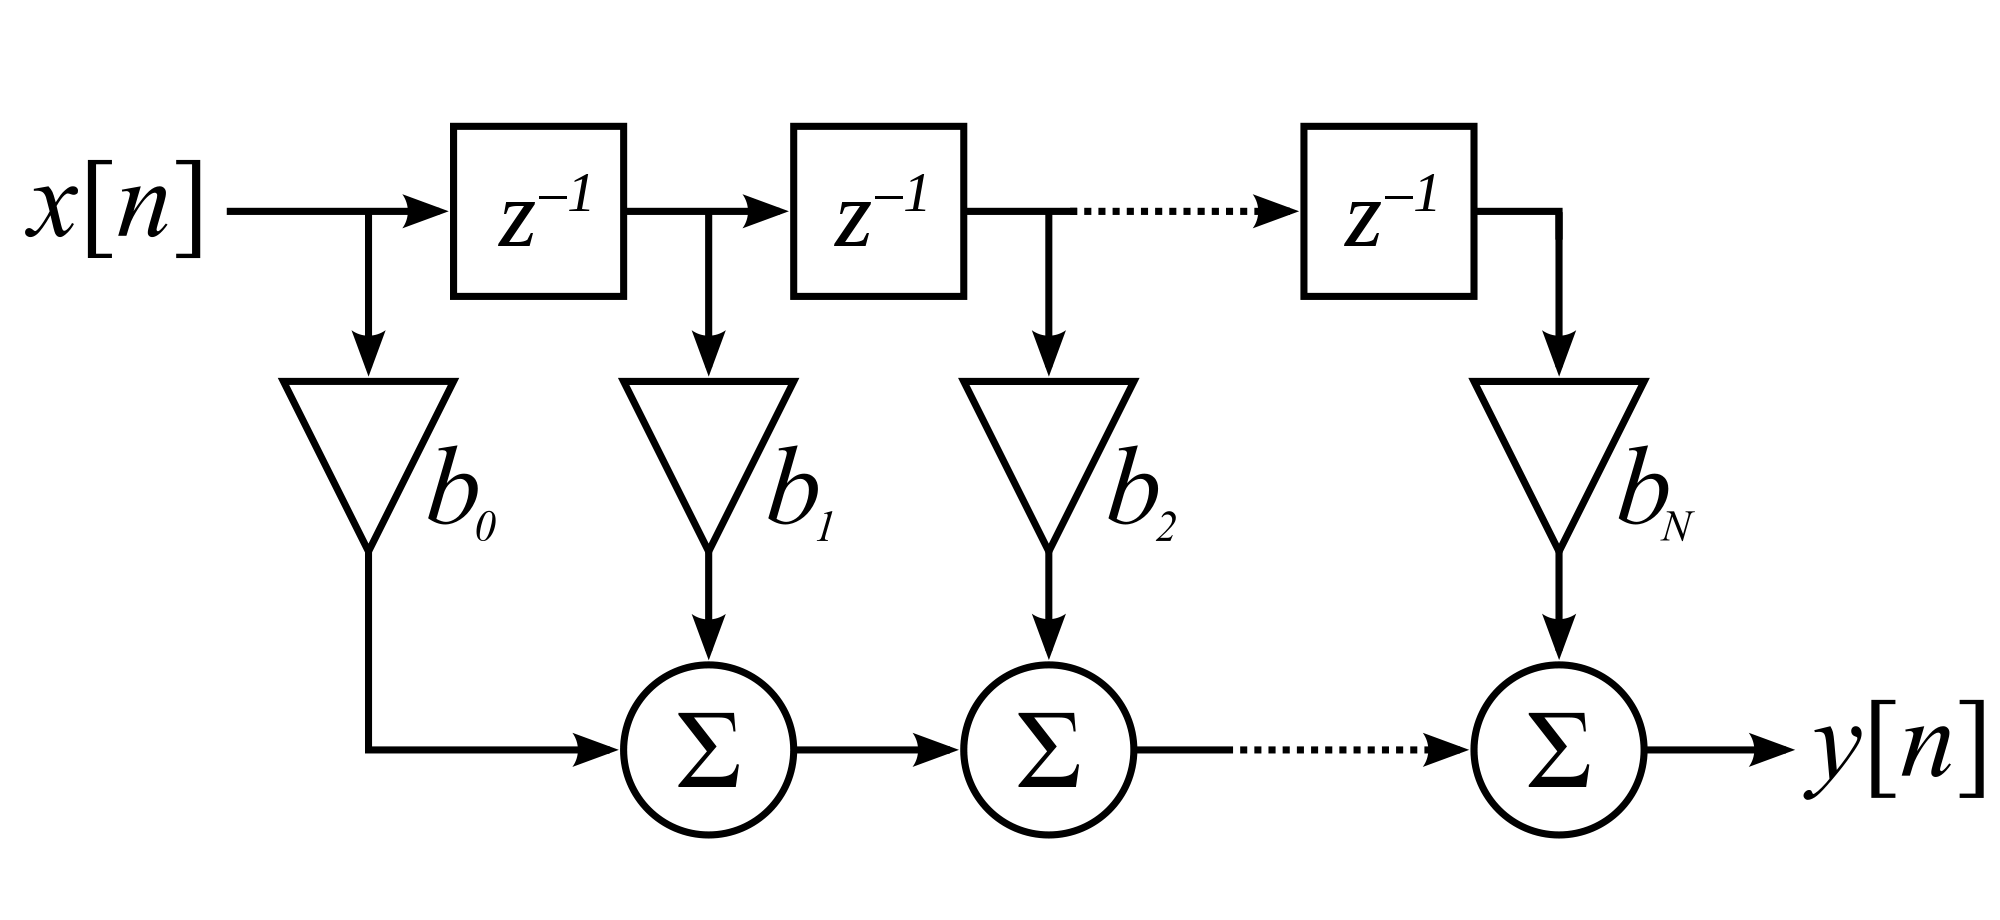
\includegraphics[width=\textwidth]{figures/fir}
			\begin{flushleft}
				\scriptsize{Image courtesy of Jonathan Blanchard, ``FIR Filter Canonical Realization,'' Wikipedia, February 23, 2008, \url{http://commons.wikimedia.org/wiki/File:FIR_Filter.svg}.}
			\end{flushleft}
		\end{column}
		\begin{column}{0.4\textwidth}
			Pros:
			\begin{itemize}
				\item Easy to implement
				\item Zero latency
			\end{itemize}
			Cons:
			\begin{itemize}
				\item Expensive if templates contain many samples
			\end{itemize}
		\end{column}
	\end{columns}
\end{frame}

\begin{frame}
	\frametitle{Frequency domain method: overlap-save}
	\begin{columns}
		\begin{column}{0.5\textwidth}
			An alternative to the time domain method is frequency domain convolution via the \textsc{fft}.

			Pros:
			\begin{itemize}
				\item Computationally efficient even for very long templates
				\item Highly tuned \textsc{fft}s available for most architectures
			\end{itemize}
			Cons:
			\begin{itemize}
				\item Input must be zero-padded, output must be clipped
				\item High latency: typically comparable to length of templates
			\end{itemize}
		\end{column}
		\begin{column}{0.5\textwidth}
			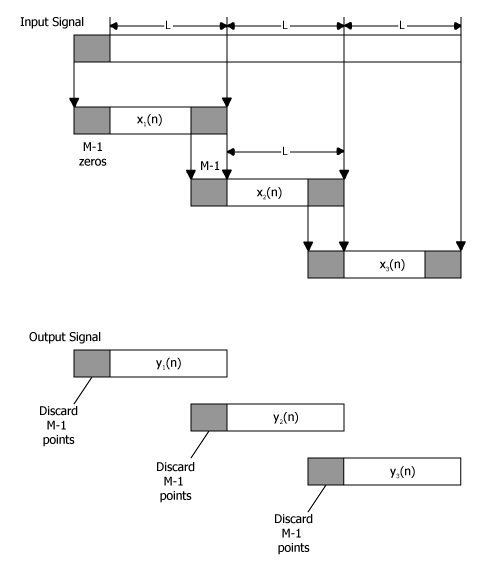
\includegraphics[width=0.9\textwidth]{figures/overlap-save}
			\begin{flushright}
				\scriptsize{Image courtesy of Douglas Jones, ``Fast Convolution,'' Connexions, June 21, 2004, \url{http://cnx.org/content/m12022/1.5/}.}
			\end{flushright}
		\end{column}
	\end{columns}
\end{frame}

\begin{frame}
	\frametitle{Frequency domain method: overlap-save}
	The frequency domain (\textsc{fd}) method's latency is determined by the overlap between blocks. \\~\\
	\begin{columns}
		\begin{column}{0.6\textwidth}
			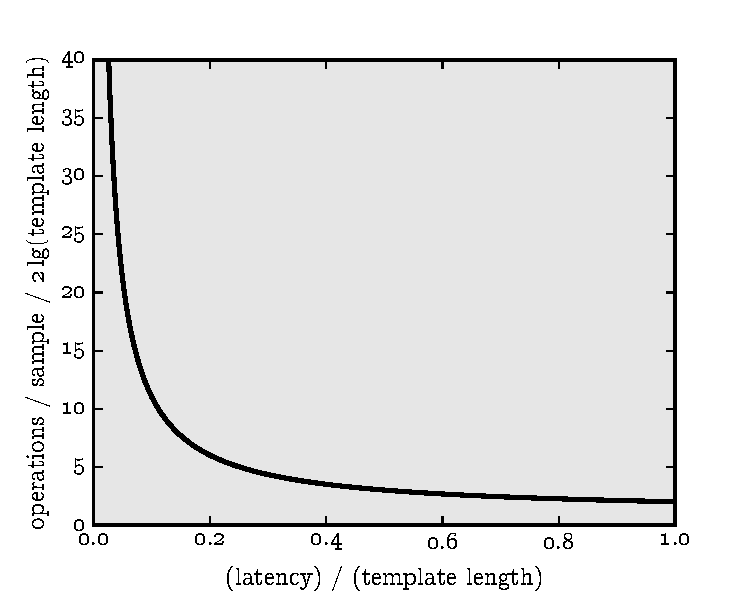
\includegraphics[width=\textwidth]{figures/fd_latency}
		\end{column}
		\begin{column}{0.4\textwidth}

			The latency can be made arbitrary small, but at the price of a {\color{ink3}\emph{divergent}} computational cost of
			\begin{equation*}
				\approx 2 \left(1 + \frac{\textrm{filter length}}{\textrm{latency}}\right)
			\end{equation*}
			operations~/~sample~/ $\lg (\textrm{template length})$.
		\end{column}
	\end{columns}
\end{frame}

\begin{frame}
	\frametitle{Novel methods can exploit properties of \textsc{cbc} signals}
	\begin{center}
		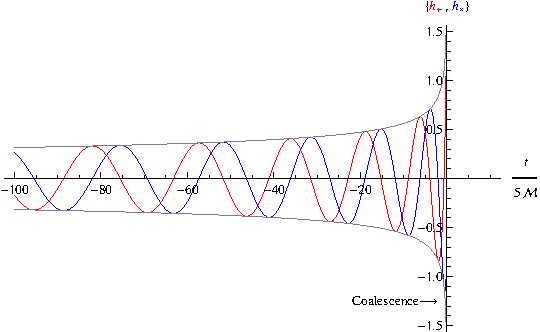
\includegraphics[width=8cm]{figures/inspiral-waveform}
	\end{center}
	\begin{itemize}
		\item Inspiral signals are chirps: ``slowly'' evolving in frequency
		\item Templates in inspiral filter banks are by design highly correlated
	\end{itemize}
\end{frame}

\begin{frame}
	\frametitle{Novel method: \textsc{lloid}}

	We exploit the chirp-like nature of inspiral signals by

	\begin{itemize}
		\item Partitioning and downsampling the template coefficients \\ \footnotesize{reducing number of filter coefficients by a factor of {\color{ink3}$\sim 10^2$}} \\~\\

		\item Decimating the detector data in several stages \\ \footnotesize{reducing sample rate by a factor of {\color{ink3}$\sim 10^2$}} \\~\\

		\item Decomposing templates further using the singular value decomposition (\textsc{svd})
		\footnotesize{reducing the number of filters by a factor of {\color{ink3}$\sim 10^1 \textrm{---} 10^2$}}
	\end{itemize}

	resulting in an overall speedup by a factor of {\color{ink3}$\sim 10^5 \textrm{---} 10^6$} over the conventional \textsc{td} method.
\end{frame}

\section[Implementation]{}

\begin{frame}
	\frametitle{First trick: time slices}

	Inspiral signals are chirps $\Rightarrow$ truncating the waveform at some time $t$ before merger results in a bandlimited signal. \\~\\

	\footnotesize{
	Using known time-frequency relationship, e.g. $f(t) = \frac{1}{\pi \mathcal{M}} \left[ \frac{5}{256}\frac{\mathcal{M}}{t}\right]^{3/8}$, \\~\\

	split templates into orthogonal ``time slices'':
	$
	\label{eq:time-slices}
	h_{i}[k] = \sum\limits_{s=0}^{S-1}
		\begin{cases}
			h_i^s[k] & \textrm{if } t^s \leqslant \frac{k}{f^0} < t^{s+1} \\
			0 & \textrm{otherwise.}
		\end{cases}
	$}

	\begin{columns}
		\begin{column}{0.5\textwidth}
			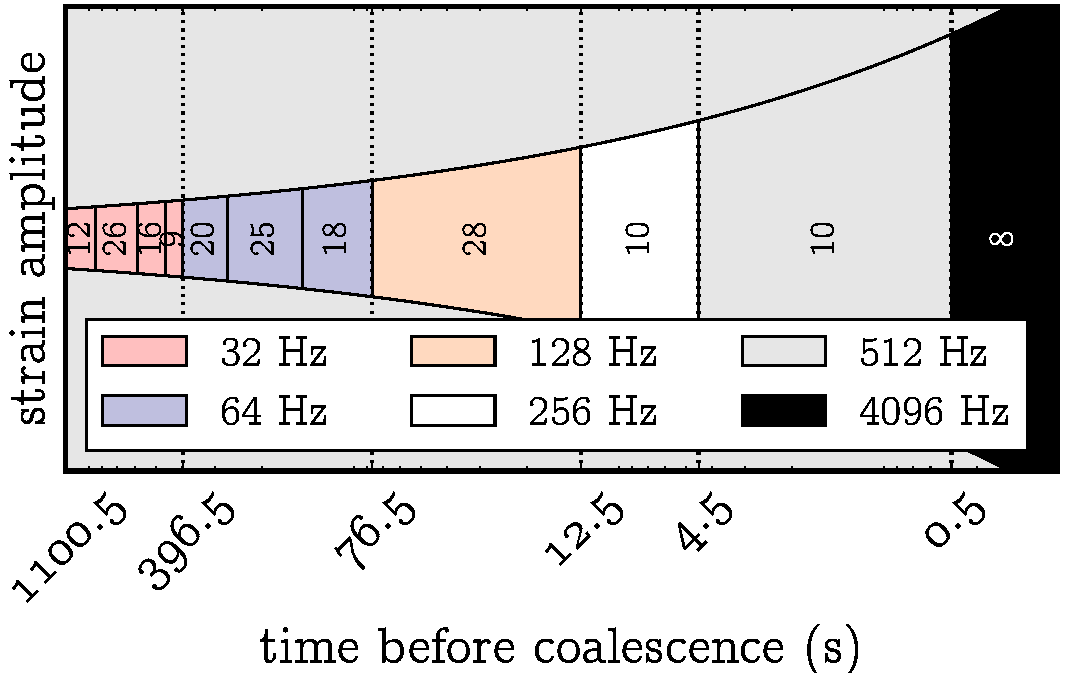
\includegraphics[width=\textwidth]{figures/envelope}
		\end{column}
		\begin{column}{0.5\textwidth}
			\footnotesize{Can downsample time slices w/o aliasing:
			$$
			h_{i}^{s}[k] \equiv
				\begin{cases}
					h_{i}\!\left[k\frac{f}{f^s}\right] & \textrm{if } t^s \leqslant k/f^s < t^{s+1} \\
					0 & \textrm{otherwise.}
				\end{cases}
			$$
			}
		\end{column}
	\end{columns}
\end{frame}

\begin{frame}
	\frametitle{Second trick: singular value decomposition}
	\begin{columns}
		\begin{column}{0.4\textwidth}
			\begin{center}
				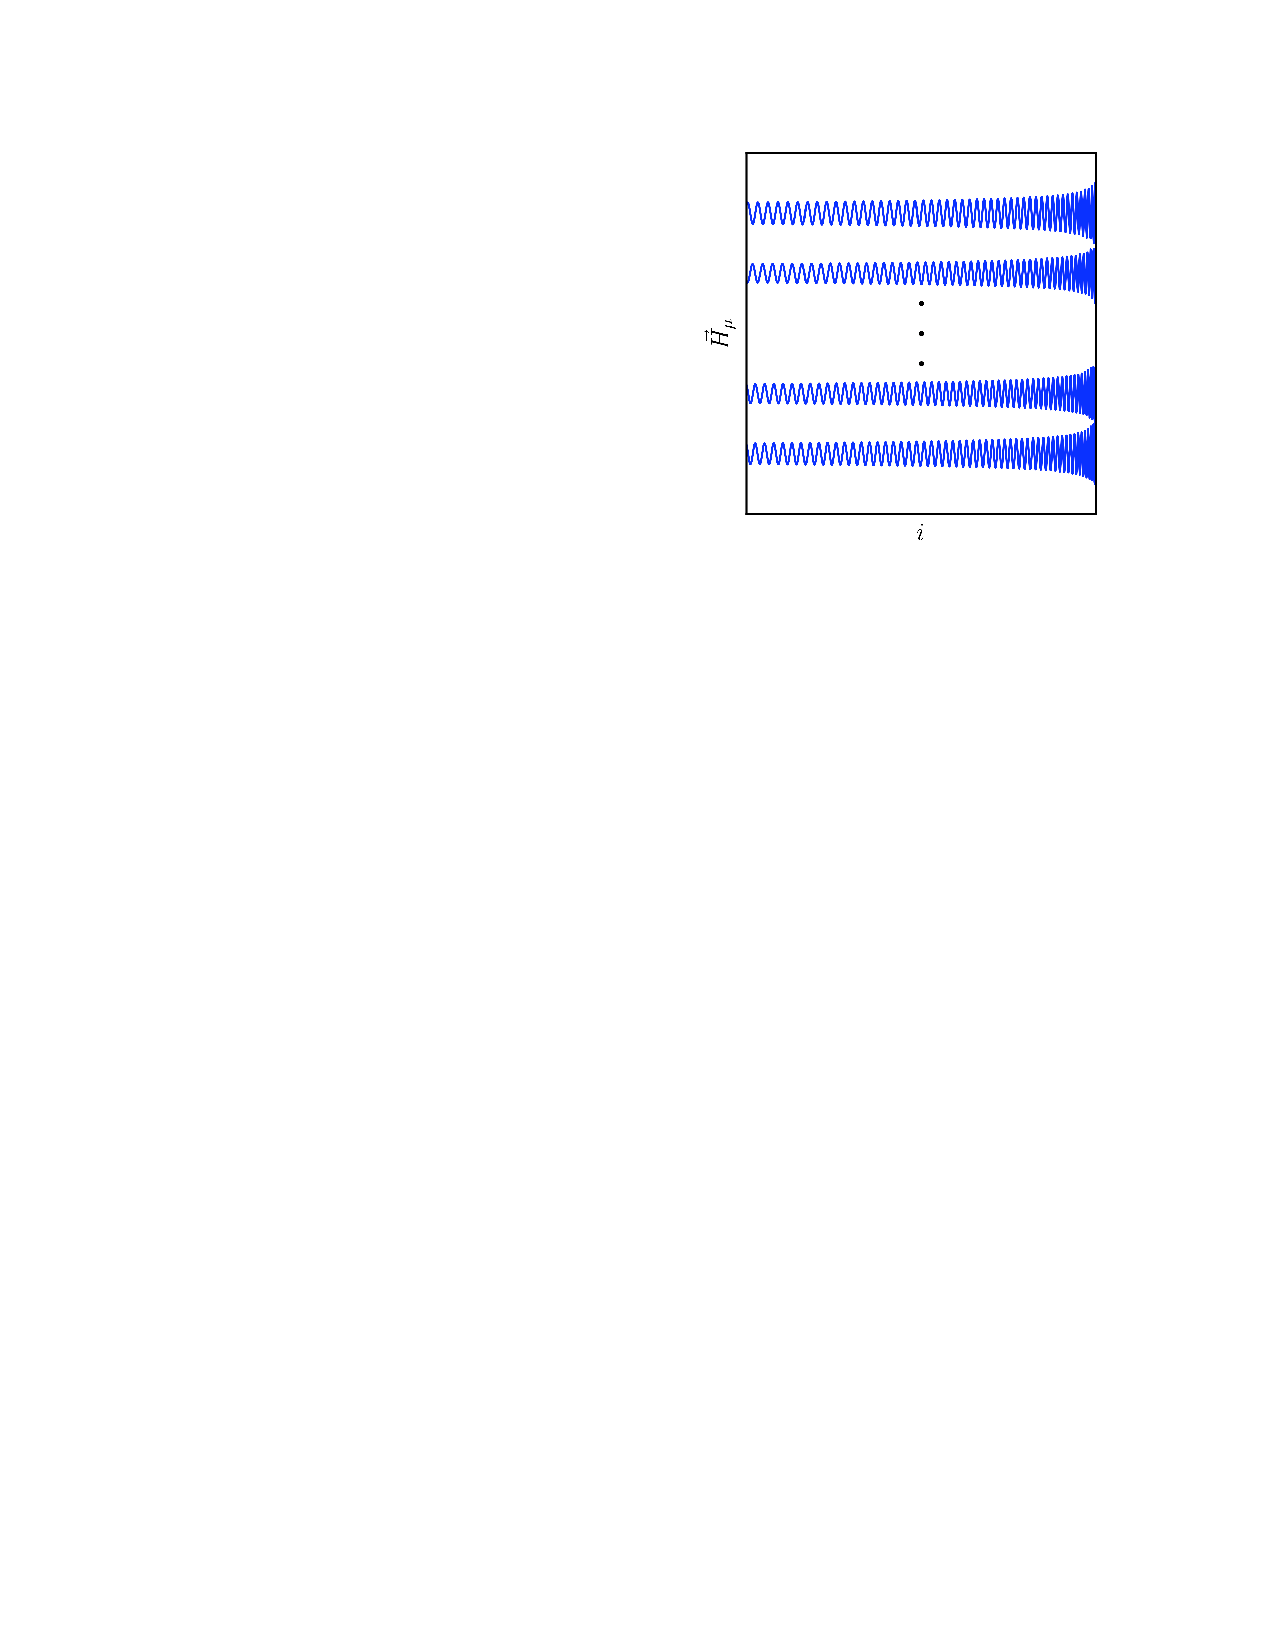
\includegraphics[width=3.5cm]{figures/original-templates}
			
				$\Downarrow$
			
				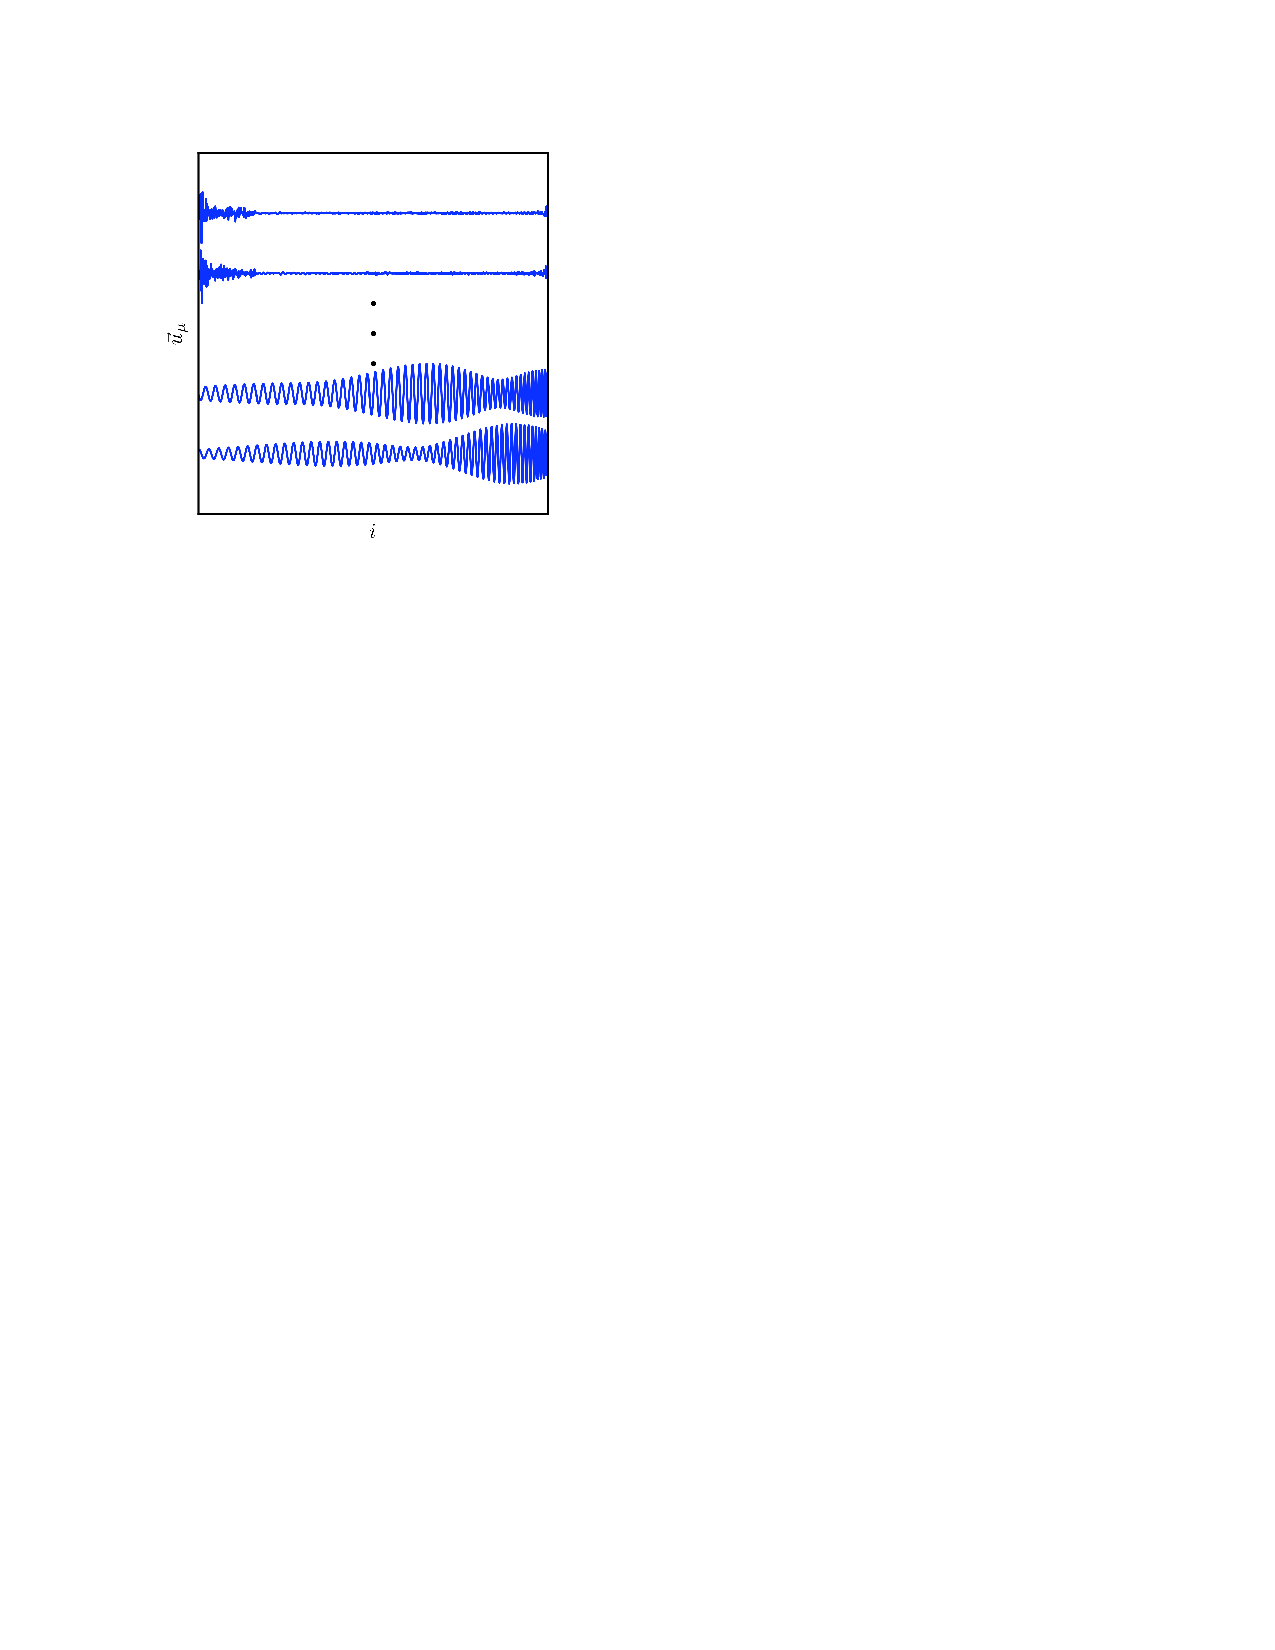
\includegraphics[width=3.5cm]{figures/svd-templates}
			\end{center}
		\end{column}
		\begin{column}{0.6\textwidth}
			Time slices represent orthogonal subspaces, but within one time slice the templates are still highly correlated. \\~\\

			We decompose the time-sliced templates further using the singular value decomposition,
			$$h_i^s[k] = \sum_{\mathclap{l=0}}^{\mathclap{M-1}} v_{il}^s \sigma_l^s u_l^s[k] \approx \sum_{\mathclap{l=0}}^{\mathclap{L^s-1}} v_{il}^s \sigma_l^s u_l^s[k].$$

			This gives us orthonormal \emph{\color{ink3}basis templates} $u_l^s[k]$, related to the original templates through a \emph{\color{ink3}reconstruction matrix} $v_{il}^s\sigma_l^s$.
		\end{column}
	\end{columns}
	\footnotesize{Images from Phys. Rev. D 82, 044025 (2010).}
\end{frame}

\begin{frame}
	\frametitle{Second trick: singular value decomposition}
	\begin{columns}
		\begin{column}{0.6\textwidth}
			The \textsc{svd} is an exact matrix factorization, but we can greatly reduce the number of filters by keeping only $L \ll M$ basis templates. \\~\\

			$L$ determines the \textsc{svd} tolerance,
			$$\left[ \sum_{l=0}^{L^s-1} \left( \sigma_l^s \right)^2 \right]\left[ \sum_{l=0}^{M-1} \left( \sigma_l^s \right)^2 \right]^{-1},$$
			which equals the expectation value of the fractional loss in \textsc{snr}.
		\end{column}
		\begin{column}{0.4\textwidth}
			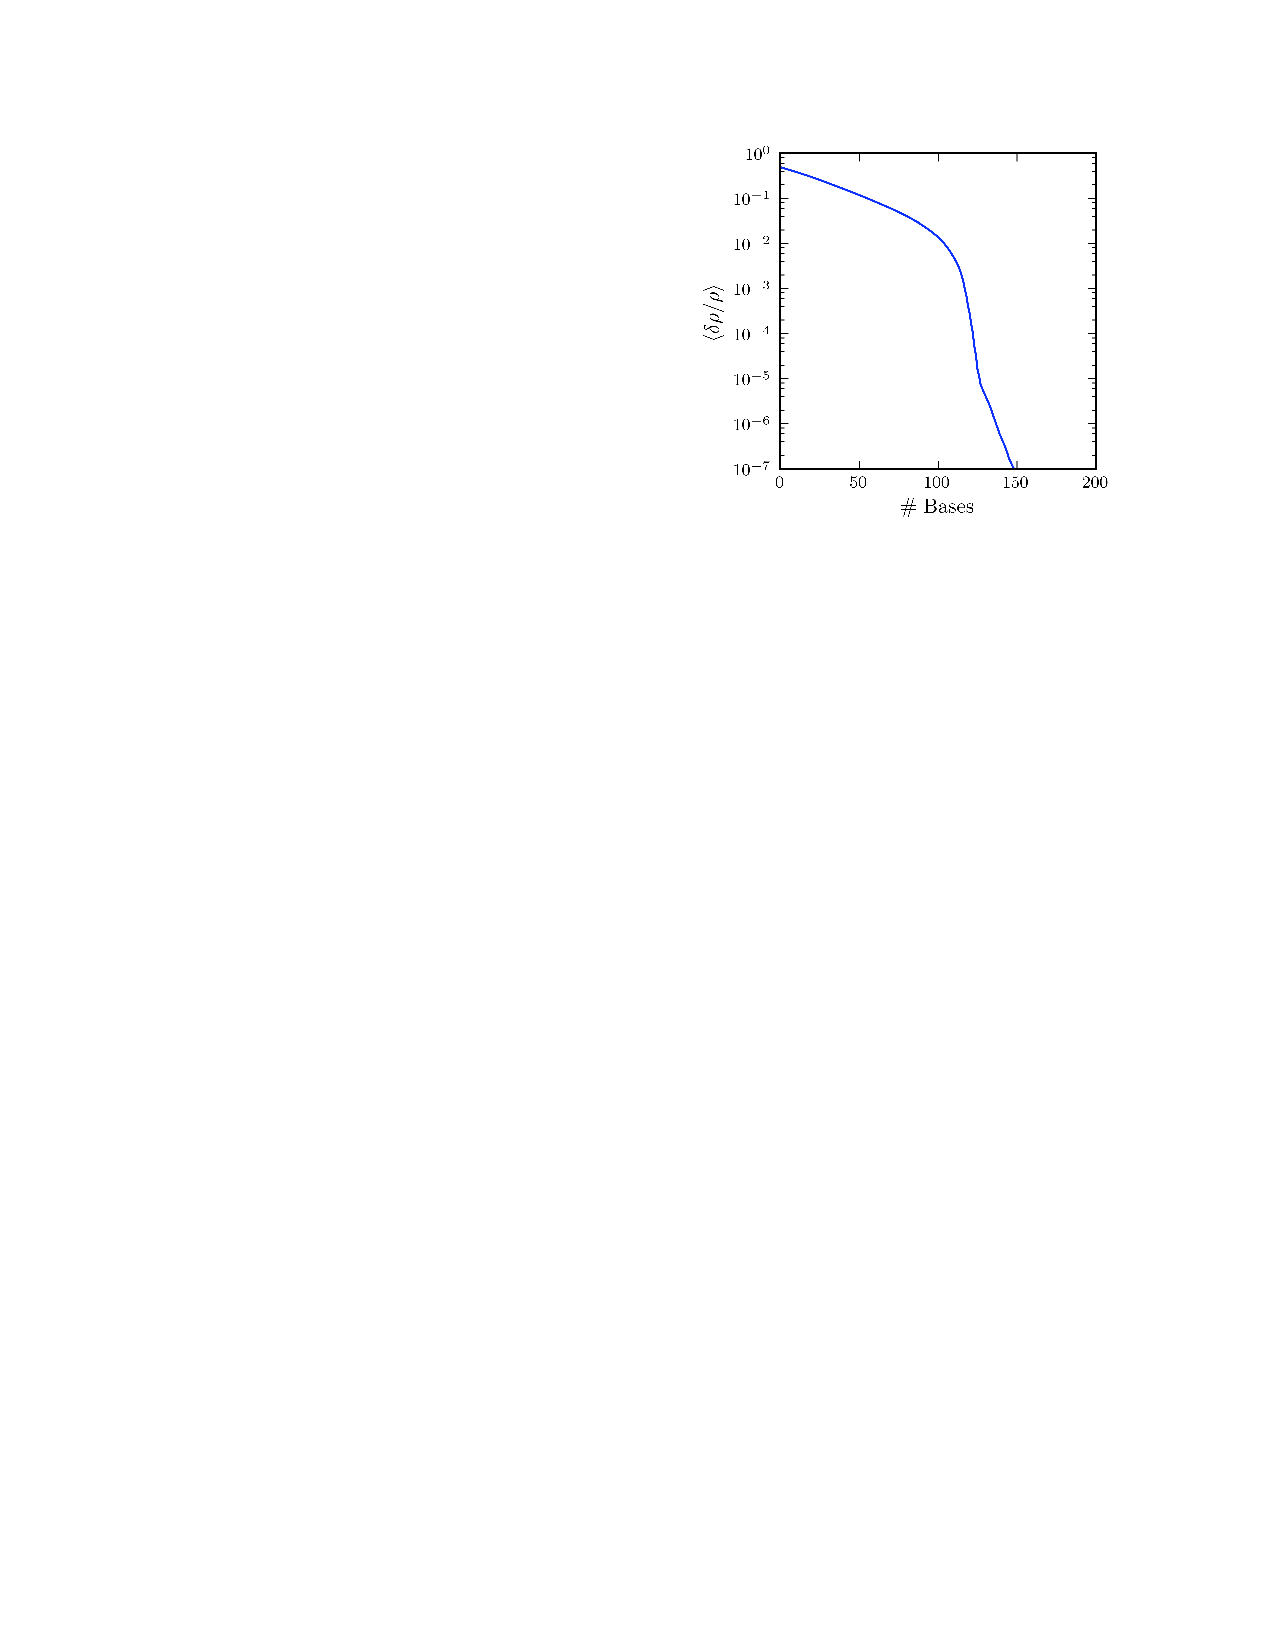
\includegraphics[width=\textwidth]{figures/singular-values}
		\end{column}
	\end{columns}
	\begin{flushright}
		\footnotesize{Image from Phys. Rev. D 82, 044025 (2010).}
	\end{flushright}
\end{frame}

\begin{frame}
	\frametitle{Implementation}
	\begin{columns}
		\begin{column}{0.5\textwidth}
			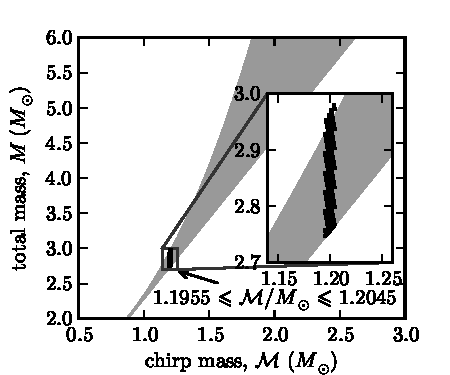
\includegraphics[width=\textwidth]{figures/tmpltbank}
		\end{column}
		\begin{column}{0.5\textwidth}
		\end{column}
	\end{columns}
\end{frame}

\begin{frame}[plain]
	\begin{center}
		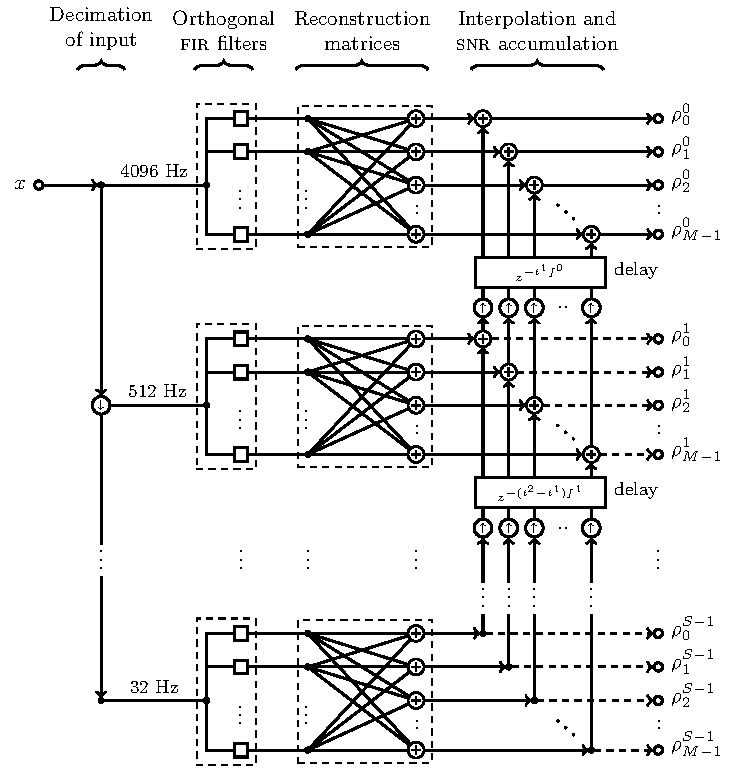
\includegraphics[height=0.75\textheight]{figures/lloid-diagram}
		\footnotesize{\begin{equation*}
			\underbrace{
				\vphantom{\Bigg(}\;\rho_i^s \; [k]\;
			}_{\raisebox{-0mm}{\text{\clap{early-warning output}}}} =%
				% Interpolation SNR
				\color{diagramaccum}
				\overbrace{
					\vphantom{\Bigg(}\left(H^\uparrow \rho_i^{s+1}\right)[k]
				}^{\raisebox{0mm}{\text{\clap{{\sc snr} from previous time slices}}}}
				% Plus ...
				\;\;+\;
				% Reconstruction
				\color{diagramreconstruct}
				\underbrace{
					\vphantom{\Bigg(}\sum_{l=0}^{L^s-1} v_{il}^s \sigma_l^s
				}_{\raisebox{-0mm}{\text{\clap{reconstruction}}}}
				% Orthogonal FIR filter
				\color{diagramfir}
				\;\;\overbrace{
					\vphantom{\Bigg(}\sum_{n=0}^{N^s-1} u_l^s[n]
					\;\color{black}
					{\smash{\underbrace{
						\vphantom{\Bigg(}x^s[k-n]
					}_{\raisebox{-0mm}{\text{\clap{decimated $h(t)$}}}}}}
				}^{\raisebox{0mm}{\text{\clap{orthogonal {\sc fir} filters}}}}
		\end{equation*}}
	\end{center}
\end{frame}

\begin{frame}
	\frametitle{GStreamer pipeline}
	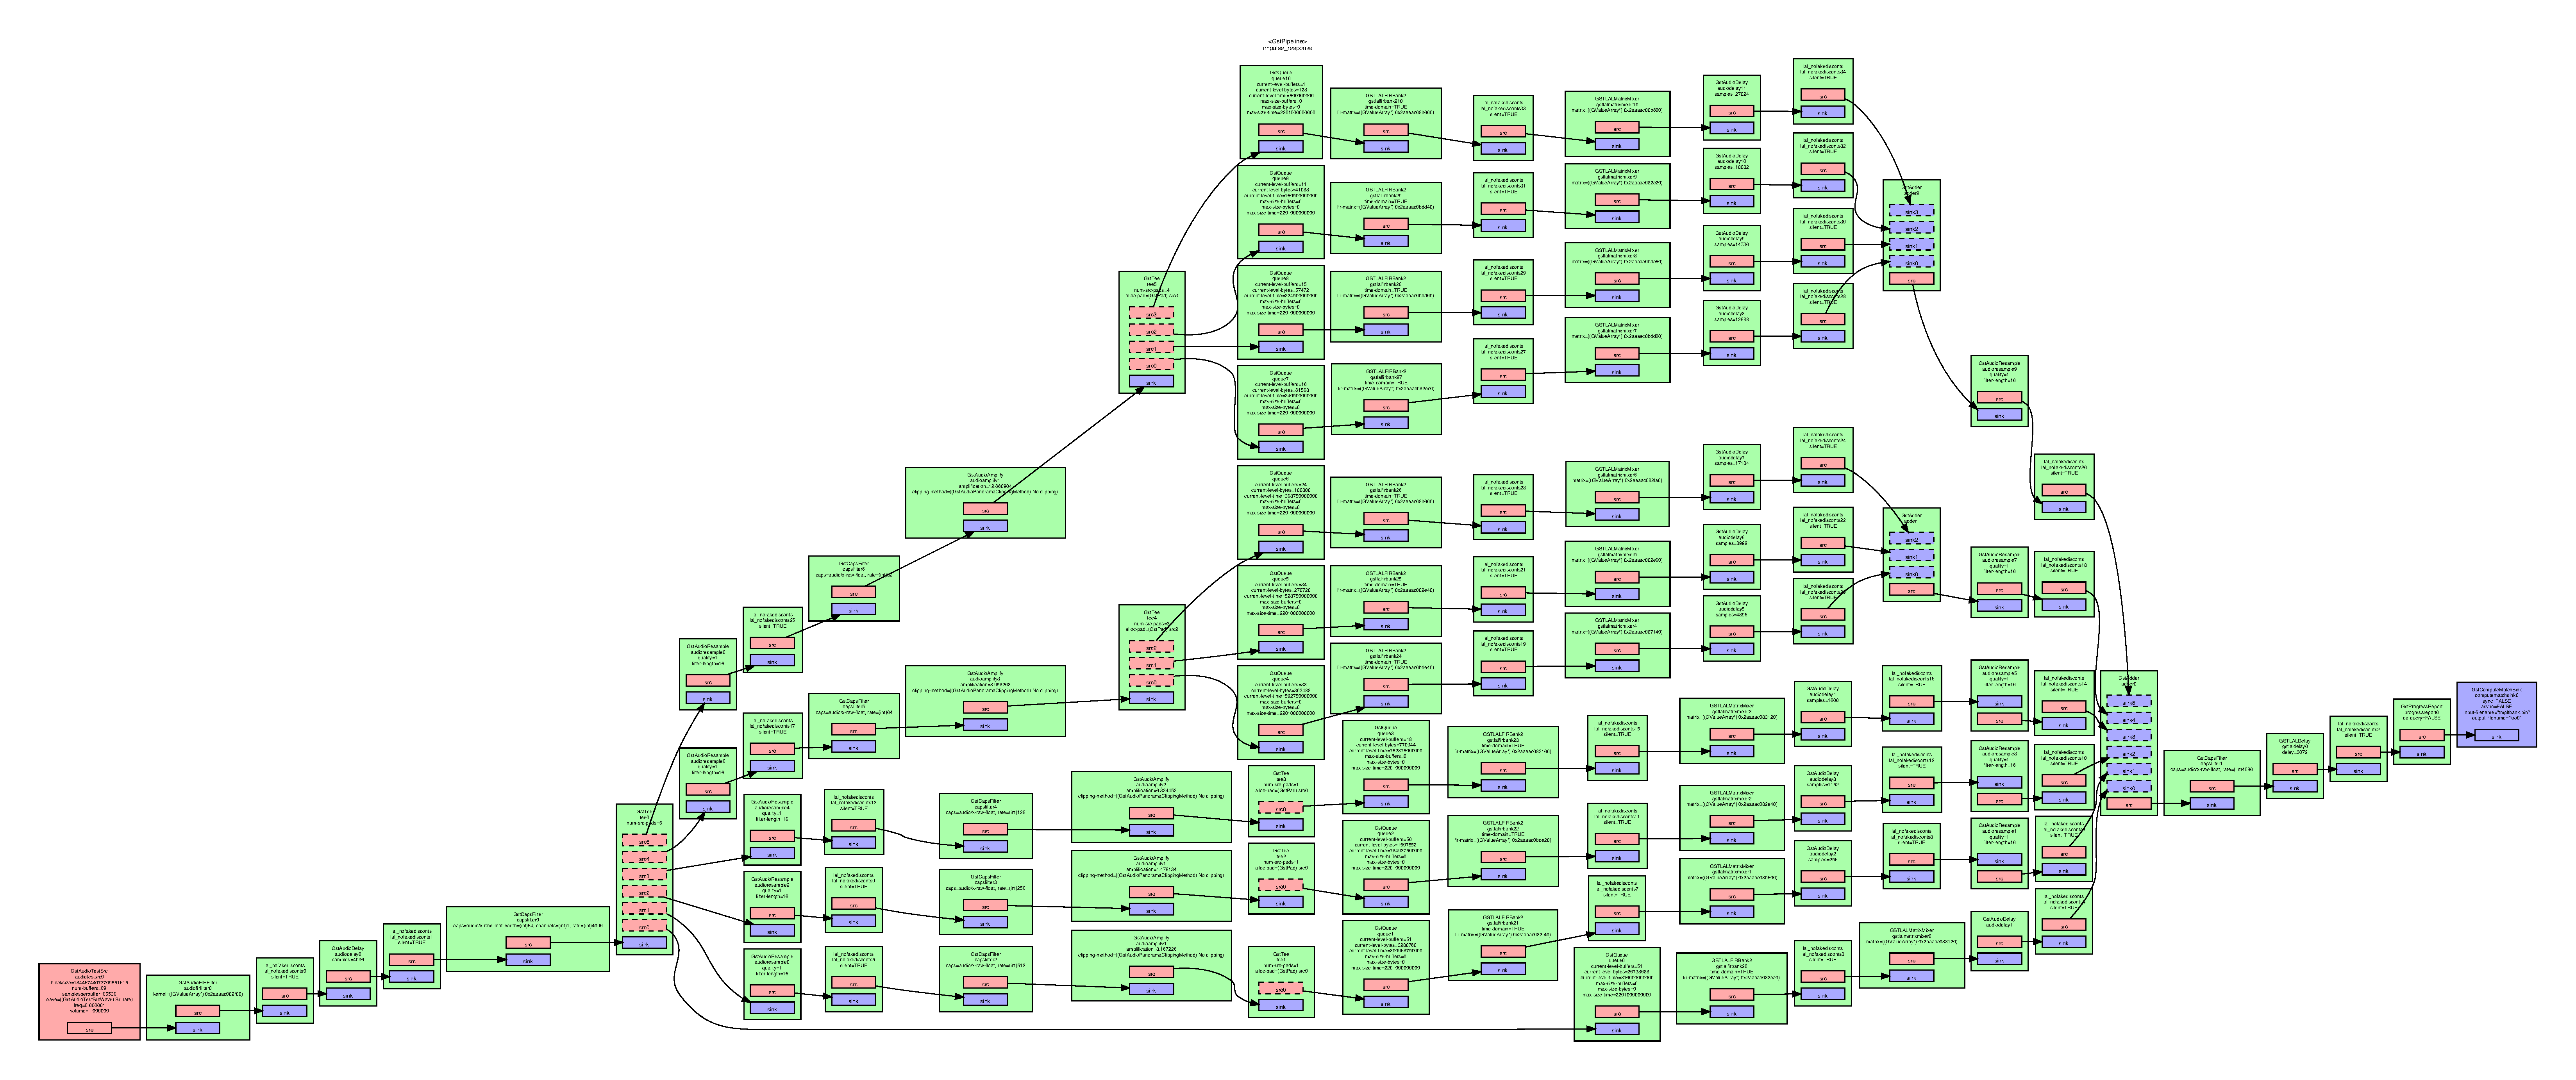
\includegraphics[width=\textwidth]{figures/pipeline}
\end{frame}

\begin{frame}
\frametitle{Computational costs and latency}
\begin{table}
\caption{\label{table:flops}Cost and latency of the \TD\ method, the \FD\ method, and \lloid.}
\begin{center}
\begin{tabular}{lll}
\hline\hline
method & \flops\ & latency (s) \\
\hline
time domain & $4.9\times10^{13}$ & 0 \\
frequency domain & $5.2\times10^8$ & $2\times10^3$ \\
\lloid\ (theory) & $4.9\times10^8$ & $2\times10^{-3}$ \\
\lloid\ (prototype) & ----------- & 5 \\
\hline
\end{tabular}
\end{center}
\end{table}

\begin{table}
\caption{Expressions for floating point operations per second (flop/s).}
\begin{tabular}{ll}
\hline\hline
method & \flops\ \\
\hline
time domain & $2 f^0 M N$ \\
frequency domain & $\approx 2 f^0 M \lg D$ \\
\lloid\ & $\approx 2 \sum_{s=0}^{S-1} f^s \numsvdtmps \left( \slicessamps + \numtmps \right)$ \\
\hline
\end{tabular}
\end{table}

\end{frame}


\section[Results]{}


\begin{frame}
\frametitle{Results}
\end{frame}


\section[Conclusion]{}


\begin{frame}
\frametitle{Conclusion}
\end{frame}

\begin{frame}
	\frametitle{Acknowledgements}
\LIGO\ was constructed by Caltech and \textsc{mit} with funding from the
\textsc{nsf} and operates under cooperative agreement
\textsc{phy}-\oldstylenums{0107417}. \textsc{ls} is supported by the
\textsc{nsf} through a Graduate Research Fellowship.
\newline\newline

\begin{center}
\scalebox{0.3}{

\includegraphics[height=3cm]{figures/LSC_logo}\hspace{7.5mm}
\raisebox{-7.5mm}{
\includegraphics[height=4.5cm]{figures/Caltech_logo}}\hspace{7.5mm}
\raisebox{-7.5mm}{
\includegraphics[height=4.5cm]{figures/nsf1}}
\raisebox{1.5mm}{\includegraphics[height=3cm]{figures/gstreamer-logo}}
}
\end{center}
\end{frame}

\end{document}
